\section{Introducción}
% TODO: insertar chamu sobre sistemas similares disponibles, etc.
En el ámbito universitario resulta necesario mantener informadas a las personas sobre una amplia variedad de hechos, noticias y acontecimientos que sucedieron o sucederán, desde la ubicación de un aula hasta la notificación de la cancelación de una clase. Muchas veces estas notificaciones son sobre cuestiones muy efímeras, lo que requiere rapidez para empezar a transmitirlas y facilidad para tener el alcance necesario.

En las facultades de la Universidad Nacional de La Plata se consumen muchos recursos para cumplir este fin, a través de afiches, pancartas, panfletos, etc. los cuales, pese a ser de barata fabricación, no tienen una vida útil muy extensa. Además todas estas formas de comunicacion se basan en el uso de papel, que tras ser utilizado debe desecharse debido a la imposibilidad de reutilizarlo, generando una cantidad de residuos significativa. Si se tiene en cuenta que también generan una polución visual considerable, por la gran cantidad de estos distribuidos en todos los lugares transitables, resulta prudente considerar una nueva forma de comunicación.

% TODO: Mencionar sobre otros carteles comercialmente disponibles
Surge así la idea de desarrollar de un cartel electrónico reutilizable, capaz de ser configurado remotamente por las autoridades competentes, con el fin de proveer una forma de comunicación masiva más limpia, clara y menos dañina para el medio ambiente.

En este informe se describe todas las fases del desarrollo de un proyecto para la asignatura Taller de Proyecto 1. El proyecto consiste en el diseño y desarrollo de un sistema de cartel luminoso cuyo contenido es configurable de forma remota. El cartel tiene conectividad WiFi, con lo que es capaz de formar parte de una red IP.

El proyecto utilizó un proceso de desarrollo de cascada, como se muestra en la figura \ref{fig:waterfall}.

\begin{figure}[!htbp]
	\centering
	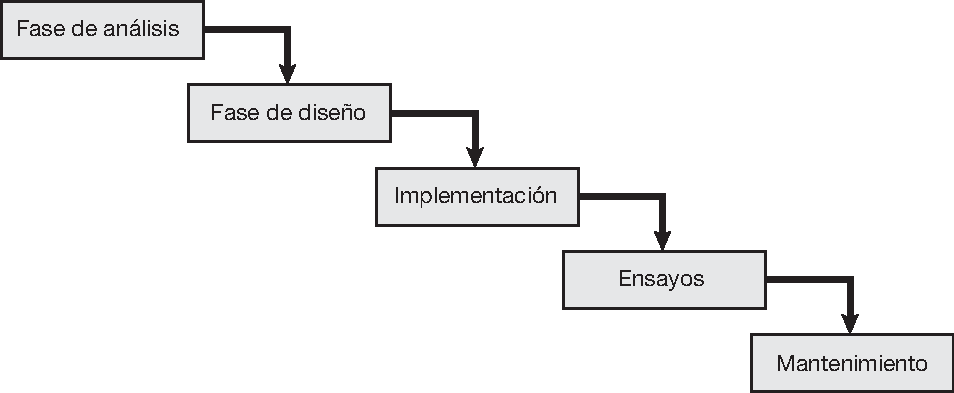
\includegraphics[width=0.8\linewidth]{imagenes/waterfall.pdf}
	\caption{Modelo en cascada de desarrollo.}
	\label{fig:waterfall}
\end{figure}

A lo largo de este informe se documentarán las fases de desarrollo previamente mencionadas.

En la sección \ref{part:analisis} se habla sobre los requerimientos y especificaciones del sistema, detallando que funcionalidades debe tener y a cuáles restricciones está sujeto.

Luego, en la sección \ref{part:diseno}, se mencionan las componentes que constituyen el sistema, se explicitan modelos que describen el comportamiento del sistema, la interfaz de usuario y la arquitectura del software. También se muestran los esquemáticos que especifican la conexión de los componentes.

En la sección de implementación se documenta como se fue dando el proceso de desarrollo de software y la implementación física del hardware.

En la sección de ensayos se documenta los resultados de las pruebas que se realizaron sobre el sistema en funcionamiento.

Por último, se anexa como apéndice una guía instructiva que explica los pasos necesarios para poner en marcha el sistema.

\section{Objetivos del proyecto}
El objetivo primario de este proyecto es el diseño implementación de un cartel luminoso que pueda ser configurado remotamente por un usuario. No se tiene como objetivo realizar un producto diseñado de manera que sea económicamente viable producirlo en masa, sino más bien el desarrollo de un prototipo a modo de prueba de concepto.

El objetivo puede ser divido en los siguientes subobjetivos:
\begin{itemize}
	\item Diseño general de la solución.
	\item Diseño e implementación del hardware que controla el cartel.
	\item Diseño e implementación del software mediante el cual se establece el contenido del cartel de forma remota.
	\item Diseño e implementación del protocolo de comunicación por el cual interactuarán las componentes.
\end{itemize}

En la parte \ref{part:analisis} se explicitará las funcionalidades que debe tener el sistema y la interfaz de usuario que expone.

\clearpage
\part{Análisis de requerimientos}\label{part:analisis}
\section{Requerimientos}
\subsection{Funcionales}
\begin{itemize}
	\item La aplicación de escritorio deberá ser capaz de poder iniciar una conexión segura con el sistema utilizando la misma para enviar los mensajes que el cliente desee.
	\item La aplicación podrá enviar peticiones de forma de obtener el mensaje actual del cartel o incluso establecer uno nuevo. Por otra parte, también podrá pedir los datos de la red a la que el sistema estará conectado o cambiarlos.
	\item La aplicación deberá ser capaz de modificar parámetros de animación tales como frecuencia de parpadeo y velocidad de desplazamiento lateral o estaticidad.
	\item La aplicación permitirá al usuario, ingresar por teclado el mensaje que desea mostrar mediante los caracteres que se establecen en el estándar de codificación de caracteres ISO/IEC 8859-1 (ver \cite{CodifChar}).
	\item El cartel deberá poder procesar sólo mensajes a través del protocolo diseñado específicamente para este proyecto (ver sección \ref{sec:protocolo})
	\item El cartel deberá mostrar los mensajes que desee el usuario.
	\item El cartel deberá poder almacenar y modificar sus credenciales de red de forma de poder conectarse al WiFi que el cliente desee.
	\item El cartel deberá mantener los datos de configuración y del mensaje que muestra, aún cuando el mismo haya sido desconectado de la red inalámbrica o de la red eléctrica.
\end{itemize}

\subsection{No funcionales}
\begin{itemize}
	\item El tiempo de respuesta del cartel no debe exceder los cinco segundos.
	\item El sistema entero no debe consumir mas de 30 Watts bajo operación normal.
	\item El sistema deberá ser capaz de aceptar sólo conexiones por TLS \cite{TLS} de forma que las conexiones y el intercambio de paquetes sea cifrado y seguro.
\end{itemize}
% TODO: Hacer diagramas de caso de uso
\subsection{Interacción con el usuario}
\section{Especificaciones físicas}
\clearpage

\part{Diseño}\label{part:diseno}
\section{Software}
\subsection{Interacción PC-Cartel}
\begin{figure}
	\centering
	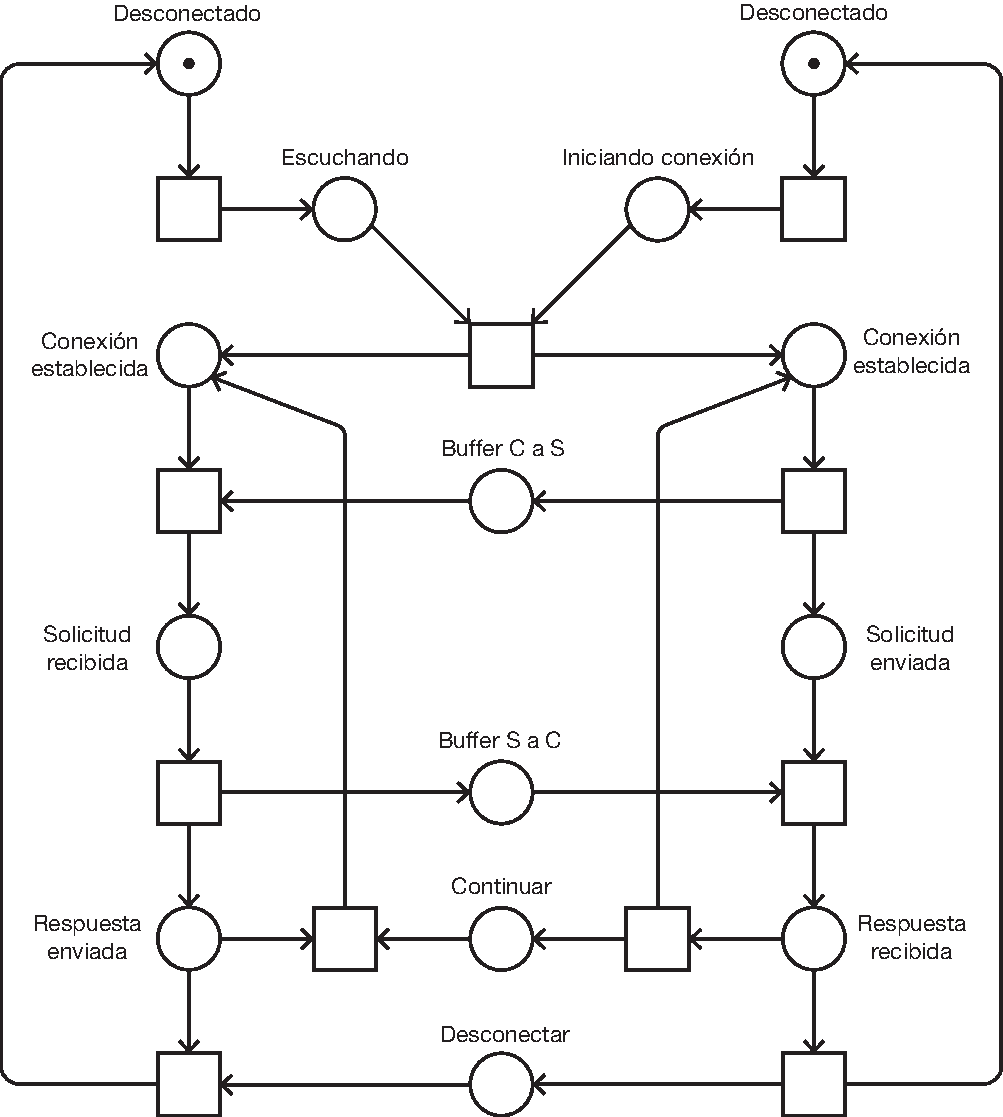
\includegraphics[width=\linewidth]{imagenes/petri-net.pdf}
	\caption{Red de Petri modelando la interacción entre la aplicación de escritorio y el cartel.}
	\label{fig:petri-net}
\end{figure}
\subsection{Firmware}
\subsubsection{Arquitectura de software}
\subsection{Aplicación de escritorio}
\subsubsection{Arquitectura de software}
\subsection{Protocolo de comunicación}\label{sec:protocolo}
\subsubsection{Transport Layer Security}

\section{Hardware}
\subsection{Diagrama en bloques general}
\subsection{Fuente de alimentación}
\subsection{Módulo maestro}
\subsection{Módulo esclavo}
\subsection{Matriz de LEDs}
\subsection{Comunicación entre los módulos}

\clearpage
\part{Ensayos y mediciones}\label{part:ensayos}
\section{Conclusiones}
% Explicar el grado de cumplimiento de objetivos planteados para el trabajo.
% Evaluar y destacar el cumplimiento y disvíos del cronograma de tareas presentados en el informe inicial
% Describir claramente la actividad de cada integrante del grupo, evaluar las horas invertidas por cada uno y calcular las horas de ingeniería total
% Analizar el presupuesto que se ha invertido y el presupuesto final del proyecto incluyendo las horas de ingeniería consumidas.